\chapter{Experimental details for DualDis}
\label{chapter:dualdisA}

\ifthenelse{\boolean{skipDual}}{\endinput}{}

\minitoc
\chapterwithfigures{\nameref*{chapter:dualdisA}}
\chapterwithtables{\nameref*{chapter:dualdisA}}


\section{Data pre-processing}

\subsection{CelebA}

The official CelebA dataset\footnote{\url{http://mmlab.ie.cuhk.edu.hk/projects/CelebA.html}} contains $\sim$200K images for 10,177 identities. As is common, we used the cropped and aligned version. However, the number of images per identity varies and some have very few images. Since our purpose is to work on datasets with two classification tasks, we chose to reduce the number of identities to 2,000, keeping those with the highest number of images. Because of this, we obtain a dataset with $\sim$60K images.

The identities are our label $\vy$ and the attributes provided with the dataset are were not preprocessed and are used as $\vz$.

\subsection{Yale-B}

The Extended Yale-B dataset\footnote{\url{http://vision.ucsd.edu/~leekc/ExtYaleDatabase/ExtYaleB.html}} is available for download in two variants: the ``full'' version contains 16128 images of 28 human subjects under 9 poses and 64 illumination conditions, each image has a large part of background; and the ``cropped'' version contains $\sim$2400 images with 38 subjects and 64 illumination conditions with no background. We chose to work with the cropped version.

The 38 identities constitute our identity label $\vy$. The lighting source information is provided as 2 real values indicating the angles (elevation and azimuth) of the light source. We propose to convert this information in 14 ``clusters'', we show the id of each cluster between 0 and 13 in this table:\\
~\\
\begin{center}
    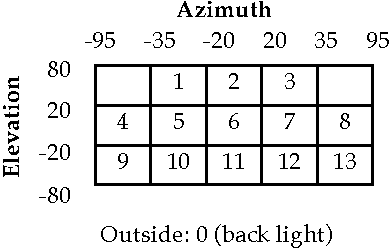
\includegraphics[width=0.45\textwidth]{images/dualdis_S_yale_cluster.pdf}
\end{center}
Each image is attributes to one of the clusters, and the label $\vz$ is a one-hot vector indicating the lighting source.

\subsection{NORB}

The NORB dataset\footnote{\url{https://cs.nyu.edu/~ylclab/data/norb-v1.0/}} ``contains images of 50 toys belonging to 5 generic categories: four-legged animals, human figures, airplanes, trucks, and cars. The objects were imaged by two cameras under 6 lighting conditions, 9 elevations (30 to 70 degrees every 5 degrees), and 18 azimuths (0 to 340 every 20 degrees).'' We use the base dataset without jitter. The 5 categories are used as our classes $\vy$, and a process similar to Yale-B is used to create the labels $\vz$, but with soft assignment:
\begin{itemize}
	\item The 6 lighting classes are converted into a single unit with values between 0 (dark) and 1 (very light) with mapping as follows: [0.6, 0.3, 0, 0.7, 0.4, 1]
	\item The elevation is represented by 3 clusters $e_i$ of centers [35, 50, 65] with an assignment to each defined as $\vz_i = 1 - \min(1, |elevation - e_i| / 15)$
	\item The azimuth is represented by 4 clusters $a_j$ of center [0, 90, 180, 270] with an assignment to each defined as $\vz_j = 1 - \min(1, |azimuth - a_j| / 9)$
\end{itemize}
This gives us a complete vector $\vz$ of size 8.

\section{Architectures \& Hyperparameters} \label{dualdisA:sec:archis_HP}

\subsection{Complete architecture overview}

To obtain the different models that we report, we use start from a complete architecture with all possible options, and then choose which parts of the model we activate. This complete architecture is represented in \autoref{dualdisA:fig:archis}.

\begin{sidewaysfigure}
    \centering
    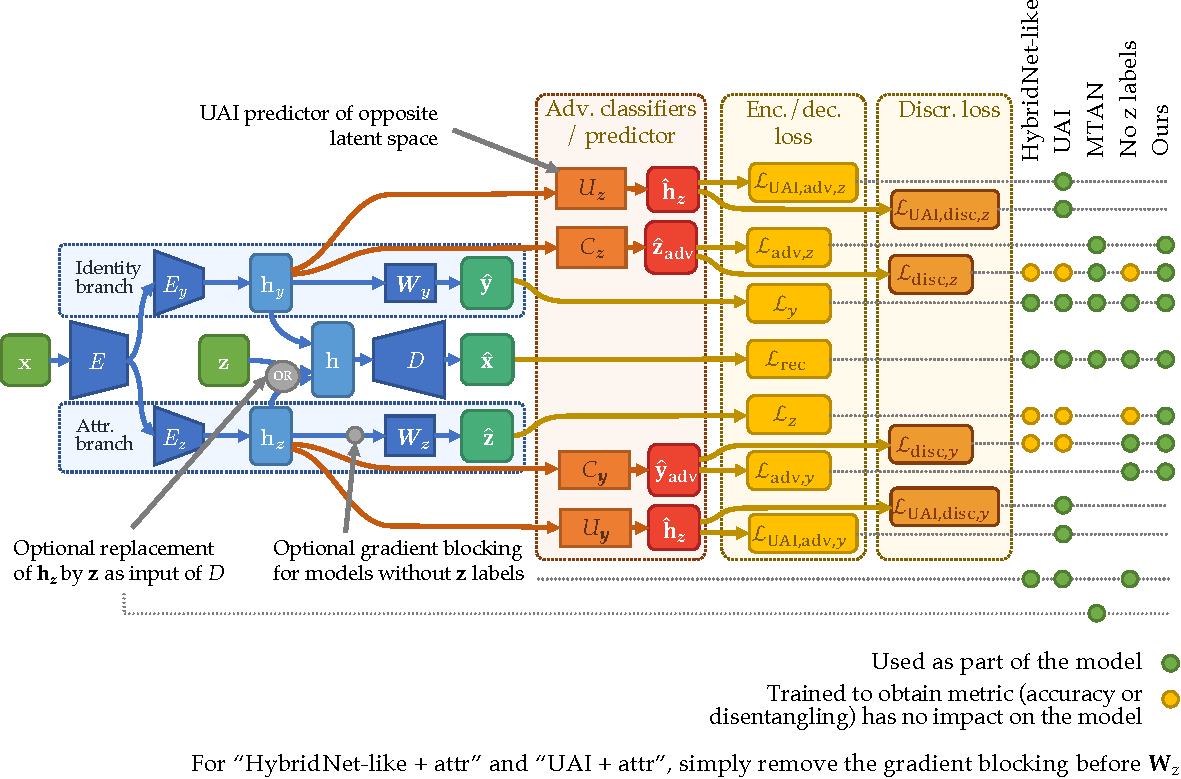
\includegraphics[width=0.92\textwidth]{images/dualdis_S_archis}
    \titlecaption{Complete architecture with all possible options and variants}{We also show which loss terms are activated to reproduce the different models that we report.}
    \label{dualdisA:fig:archis}
\end{sidewaysfigure}

In particular, we can see that we have:
\begin{itemize}
    \item $U_y$ and $U_z$ which are the predictors that replace $C_y$ and $C_z$ for UAI model, and that predict $\vhy$ and $\vhz$. Their corresponding loss term is a MSE for both $\calL_\textrm{UAI,adv}$ and $\calL_\textrm{UAI,disc}$ that is maximized for $\calL_\textrm{UAI,adv}$ and minimized for $\calL_\textrm{UAI,disc}$.
    \item The possibility to replace $\vhz$ by $\vz$ as the second input of the decoder $D$, which allows to produce MTAN.
    \item The possibility to block gradients between $\vhz$ and $\vW_z$, which means that when activated we can train $\vW_z$ to measure the quality of the representation $\vhz$ regarding the attributes, while not backpropagating this signal to $E_z$, therefore reproducing models that do not use $\vz$ labels while keeping the metric.
    \item It is possible to train adversarial classifiers $C_y$ and $C_z$ with $\calL_\textrm{disc}$ even when not proposed by the models, which allows to measure the quality of the disentangling and will have no impact of the actual model as long as $\calL_\textrm{adv}$ are disabled since $\calL_\textrm{disc}$ is only backpropagated in $C$.
\end{itemize}

\clearpage

\subsection{Architecture details}

In \autoref{dualdisA:tab:archis}, we provide the exact details about the architecture of the components in \autoref{dualdisA:fig:archis} depending on the experiments and the dataset, along with those general information:


\newcommand{\nlspace}{\rule{0pt}{9pt}}
\newcommand{\li}{$\ell$}

\begin{itemize}
    \item In the \textbf{encoder}, every layer is followed by batch normalization and ReLU.
    \item In the \textbf{decoder}, every layer is followed by a batch normalization and Leaky\-ReLU(0.2), except last layer which has no activation or BN.
    \item In the \textbf{classifiers}, every intermediate layer is followed by a ReLU.
    \item \textbf{Layers are described using the following syntax:}
    \begin{itemize}
    \item \textbf{Conv:} \texttt{128[k5][p0][s2]} is a convolutional layer with 128 output channels, a kernel of 5 (default is 3 if not written), padding of 0 (default is to keep same output size), stride 2 (default is 1)
    \item \textbf{Deconv:} \texttt{dec128[k4][p0][s1]} is a transpose convolutional layer with 128 output channels, a kernel of 4 (default), padding of 0 (default is 1), stride 1 (default is 2)
    \textbf{Linear:} \li\texttt{128} is a linear layer with 128 output neurons
    \item \textbf{Upsample:} \texttt{upsample} means an upsampling of a factor 2 using the nearest value  
    \item \textbf{MaxPool:} \texttt{maxpool2k3} is a max-pooling of stride 2 and kernel 3
    \end{itemize}
\end{itemize}

\begin{table}[p]
    \centering
    \begin{tabular}{r|p{0.41\textwidth}|p{0.41\textwidth}}
        \toprule
         & Architecture for UAI & Architecture for all other models \\
        \midrule
        \multicolumn{3}{c}{\textbf{CelebA} (image size 256$\times$256)}\\
        \midrule
        
       $E$
       & 32p0s2, 32p0s1, 64p0, maxpool2k3, 80k1, maxpool2k3, 96p0, maxpool2k3, 128p0, 160p0s2, 196p0
       & 32p0s2, 32p0s1, 64p0, maxpool2k3, 80k1, maxpool2k3, 96p0, maxpool2k3
       \\ \nlspace
       $E_y/E_z$
       & 196p0
       & 96p0, 128p0s2, 196p0, 196p0
       \\ \nlspace
       $D$
       & \multicolumn{2}{p{0.82\textwidth}}{dec392p0s1, 392, upsample, 392, upsample, 256, upsample, 196, upsample, 128, 128, upsample, 96, 96, upsample, 64, 64, 32, 3k1}
       \\ \nlspace
       $\vW_y$ & \li2000 & \li2000 \\ \nlspace
       $\vW_z$ & \li40 & \li40 \\ \nlspace
       $C_y$ & \li256, \li2000 & \li256, \li256, \li2000 \\  \nlspace
       $C_z$ & \li256, \li40 & \li256, \li256, \li40 \\ \nlspace
       $U_y$ & \li196 & N/A \\\nlspace
       $U_z$ & \li196 & N/A \\
        
        
        \midrule
        \multicolumn{3}{c}{\textbf{Yale-B} (image size 64$\times$64)}\\
        \midrule
        
       $E$
       & 32k4s2, 40k4s2, 48k4s2, 76k4s2, 100k3p0
       & 32k4s2, 40k4s2, 48k4s2
       \\ \nlspace
       $E_y/E_z$
       & 80k2p0
       & 64k4s2, 72k3p0, 80k2p0
       \\ \nlspace
       $D$
       & \multicolumn{2}{p{0.82\textwidth}}{160k2p1, dec80, dec64, dec48, dec32, dec32, 32, 3none}
       \\ \nlspace
       $\vW_y$ & \li38 & \li38 \\ \nlspace
       $\vW_z$ & \li14 & \li14 \\ \nlspace
       $C_y$ & \li80, \li80, \li38 & \li80, \li80, \li38 \\  \nlspace
       $C_z$ & \li80, \li80, \li14 & \li80, \li80, \li14 \\ \nlspace
       $U_y$ & \li80 & N/A \\\nlspace
       $U_z$ & \li80 & N/A \\
        
        
        \midrule
        \multicolumn{3}{c}{\textbf{NORB} (image size 64$\times$64)}\\
        \midrule
        
       $E$
       & 64k4s2, 64k4s2, 96k4s2, 164k4s2, 192k4s2
       & 64k4s2, 64k4s2, 96k4s2
       \\ \nlspace
       $E_y/E_z$
       & 128k2p0
       & 96k4s2, 128k3p0, 128k2p0
       \\ \nlspace
       $D$
       & \multicolumn{2}{p{0.82\textwidth}}{256k2p1, dec192, 128, dec128, 128, dec96, 96, dec64, 64, dec64, 64, 32, 1}
       \\ \nlspace
       $\vW_y$ & \li5 & \li5 \\ \nlspace
       $\vW_z$ & \li8 & \li8 \\ \nlspace
       $C_y$ & \li128, \li128, \li5 & \li128, \li128, \li5 \\  \nlspace
       $C_z$ & \li128, \li128, \li8 & \li128, \li128, \li8 \\ \nlspace
       $U_y$ & \li128 & N/A \\\nlspace
       $U_z$ & \li128 & N/A \\
        
        \bottomrule
    \end{tabular}
    \titlecaption{Architectures used for our experiments}{\newline\newline}
    \label{dualdisA:tab:archis}
\end{table}





\subsection{Training and hyperparameters values}

As a reminder, we have two losses composed of different loss terms, each weighted by a parameter $\lambda$ that controls its importance. Here is the global loss:
\begin{align}
\calL_\mathrm{main} &= \lambda_{rec} \calL_\textrm{rec} + \lambda_y \calL_{y} + \lambda_z \calL_{z} + \lambda_{adv,y} \calL_{\textrm{adv},y} + \lambda_{adv,z} \calL_{\textrm{adv},z} + \lambda_{o} \calL_\textrm{orth}\,.\\
\calL_\mathrm{disc} &= \lambda_{disc,y} \calL_{\textrm{disc},y} + \lambda_{disc,z} \calL_{\textrm{disc},z}\,.
\end{align}

This loss is optimized using Adam with the recommended hyperparamters: learning rate of $0.001$, $\beta_1 = 0.9$, $\beta_2 = 0.999$. The number of epochs and batch sizes depends on the datasets and are given below.

For all the experiments, we used $\lambda = 1$ for all the classification losses:
$\lambda_y = \lambda_z = \lambda_{disc,z} = \lambda_{disc,z} = \lambda_{UAI,disc,z} = \lambda_{UAI,disc,z} = 1$, and we set $\lambda_{o} = 1\times 10^{-6}$

Values of hyperparameters that depends on the dataset are provided in \autoref{dualdisA:tab:HP}.

\begin{table}[H]
    \centering
    \begin{tabular}{rcccccccccccc}
        \toprule
        & $\lambda_{rec}$ & $\lambda_{adv,y}$ & $\lambda_{adv,z}$ & $\lambda_{UAI,adv,y}$ & $\lambda_{UAI,adv,z}$ & Batch size & Epochs \\
        \midrule
        CelebA       & 0.3 & 0.1  & 0.1  & 0.3 & 0.3 & 32 & 330 \\
        %CelebA AS    & 0.3 & 0.1  & 0.25 & -   & -   & 32 & 330 \\
        Yale-B        & 1   & 0.08 & 0.08 & 0.3 & 0.3 & 64 & 400 \\
        %Yale AS     & 1   & 0.08 & 0.08 & -   & -   & 64 & 400 \\
        NORB         & 10  & 0.25 & 0.25 & 0.3 & 0.3 & 128 & 250 \\
        %NORB AS     & 10  & 0.25 & 0.25 & -   & -   & 128 & 250 \\
        \bottomrule
    \end{tabular}
    \titlecaption{Hyperparameters for the various experiements}{}
    \label{dualdisA:tab:HP}
\end{table}

\section{Experiments details}

\subsection{Image editing}

For image editing, we use the model trained for the ablation study of the datasets, and start by obtaining the representations $\vhy$ and $\vhz$ for some test images. For attribute modification, we move $\vhz$ in the direction $i$ of each vector $\vw_{z_i}$ to obtain $\vhz' = \vhz \pm \varepsilon \vw_{z_i}$ of the model and produce images using the decoder: $\vxh = D(\vhy, \vhz')$. The amplitude of $\varepsilon$ for the visualization was fixed after a quick visual check of what values looked.
For identity / attributes mixing between images, we simply use $\vhy$ and $\vhz$ from different images and feed them to the decoder.

\subsection{Semi-supervised learning}

For semi-supervised learning, we use batches with a pre-defined number of supervised images in each batch. We iterate over the set of labeled and unlabeled images independently and consider an epoch as the loop over the unlabeled image set, during which we usually see images of the supervised set more than once depending on the size of the sets. This is a common setting, e.g. \citep{Sajjadi2016,tarvainen2017mean,Robert2018}. The hyperparameters that differ from the model in the ablation study are provided in \autoref{dualdisA:tab:HP_SSL}.

\begin{table}[H]
    \centering
    \begin{tabular}{rcccccccccccc}
        \toprule
        & $\lambda_{rec}$ &  $\lambda_{z}$ & $\lambda_{adv,y}$ & $\lambda_{adv,z}$ & Sup. batch size \\
        \midrule
        4000     & 0.3 & 0.4 & 0.2  & 0.1 & 10 \\
        2000     & 0.5 & 0.4 & 0.2  & 0.1 & 10 \\
        1000     & 0.5 & 0.4 & 0.2  & 0.1 & 8 \\
        400      & 0.5 & 0.4 & 0.2  & 0.1 & 8 \\
        
        \bottomrule
    \end{tabular}
    \titlecaption{Hyperparameters for the \acs{SSL} experiements}{``Sup. batch size'' indicates the number of labeled images in each batch.}
    \label{dualdisA:tab:HP_SSL}
\end{table}


\subsection{Data Augmentation on Yale-B}

For the \acf{DA} experiments, we start by training a new model with different sizes of train datasets. Once trained, we produce 150 new images for each identity using the image editing technique we described in order to produce new images of the different attribute categories. For this, we iterate over the train images of each identity (after excluding train images with attributes that correspond to very bad lighting, \textit{i.e.} attributes 0, 4, 8, 9, 13) and then randomly choose an attribute for which we do not already have enough images for this identity. This is done so that after \ac{DA}, each identity has images that follows this distribution $\mathcal D$ over attributes 0 to 13:
\begin{equation}
    \mathcal D = [1, 3, 3, 2, 5, 3, 10, 3, 5, 2, 2, 2, 2, 2] / 45
\end{equation}

Then, a classifier with the architecture $\vW_y \circ E_y \circ E$ is trained with Adam for 400 epochs on the original train set used for to train the generator + the generated images. It is then evaluated on all the remaining images of the original dataset.
